\section{Versuchsaufbau und Durchf"uhrung} % (fold)
\label{sec:durchfuehrung}

\subsection{Direkte Messung der Leerlaufspannung} % (fold)
\label{sub:direkte_messung_der_leerlaufspannung}

\begin{wrapfigure}{r}{7cm}
	\centering
	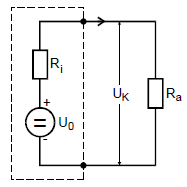
\includegraphics[width = 5cm]{img/Monozelle.PNG}
	\caption{Schaltbild zur direkten Messung der Leerlaufspannung. \cite{anleitung}}
	\label{aufgabea}
\end{wrapfigure}{r}

Die Schaltung wird nach Abb.\ref{aufgabea} aufgebaut. Der Widerstand $R_\mathrm{a}$ entspricht hierbei dem Eingangswiderstand $R_\mathrm{v}$ des hochohmigen Spannungsmessger"ates.
Es werden $U_\mathrm{k}$ und $R_\mathrm{v}$ notiert.

\newpage

\subsection{Messung der Leerlaufspannung und des Innenwiderstandes mittels eines variablen Widerstandes} % (fold)
\label{sub:messung_der_leerlaufspannung_mittels_eines_variablen_widerstandes_}

\begin{wrapfigure}{r}{7cm}
	\centering
	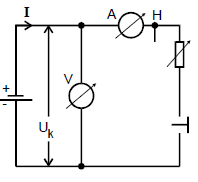
\includegraphics[width = 5cm]{img/b.PNG}
	\caption{Messchaltung zur Bestimmung von $U_\mathrm{0}$ und $R_\mathrm{i}$ \cite{anleitung}.}
	\label{aufgabeb}
\end{wrapfigure}{r}

Die Schaltung wir nach Abb.\ref{aufgabeb} aufgebaut.
Der variable Belastungswiderstand liegt dabei in einem Bereich von $\SI{0}{\ohm}$ bis $\SI{50}{\ohm}$. Es werden bei 10 verschiedenen Belastungswiderst"anden $R_\mathrm{k}$ die Klemmenspannung $U_\mathrm{k}$ in Abh"angigkeit von dem Belastungsstrom $I$ aufgenommen.

\subsection{Messung der Leerlaufspannung und des Innenwiderstandes mittels eines variablen Widerstandes und einer Gegenspannung} % (fold)
\label{sub:messung_der_leerlaufspannung_mittels_eines_variablen_widerstandes_}

\begin{wrapfigure}{r}{7cm}
	\centering
	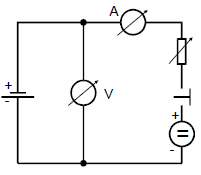
\includegraphics[width = 5cm]{img/c.PNG}
	\caption{Messchaltung zur Bestimmung von $U_\mathrm{0}$ und $R_\mathrm{i}$ mittels einer Gegenspannung \cite{anleitung}.}
	\label{aufgabec}
\end{wrapfigure}{r}

Die Schaltung wird nach Abb.\ref{aufgabec} aufgebaut.
Die Gegenspannung soll dabei etwa $\SI{2}{\volt}$ gr"o"ser sein als die Leerlaufspannung $U_\mathrm{0}$.
Es werden bei 10 verschiedenen Belastungswiderst"anden $R_\mathrm{k}$ die Klemmenspannung $U_\mathrm{k}$ in Abh"angigkeit von dem Belastungsstrom $I$ aufgenommen.

\subsection{Sinus- und Rechteckausgang} % (fold)
\label{sub:sinus_und_rechteckausgang}

Die Schaltung wird nach Abb.\ref{aufgabeb} aufgebaut.
Nun wird jedoch ein Sinus- bzw. Rechtecksspannungsgenerator angeschlossen.

F"ur die Messung mit der Rechtecksspannung wird ein variabler Widerstand von $\SI{20}{\ohm}$ bis $\SI{250}{\ohm}$ benutzt.

Bei der Messung mit der Sinusspannung hingegen einer mit einem Bereich von $\SI{0.1}{\kilo\ohm}$ bis $\SI{5}{\kilo\ohm}$.

Es werden bei 10 verschiedenen Belastungswiderst"anden $R_\mathrm{k}$ die Klemmenspannung $U_\mathrm{k}$ in Abh"angigkeit von dem Belastungsstrom $I$ aufgenommen.